\chapter{Implementing the method}

\subsection{CGAL}
To develop the method seen previously, we chose to use CGAL (Computational Geometry
 Algorithms Library) \cite{CGAL}.
CGAL is a software project which supplies a free access with numerous effective
 and reliable geometrical algorithms in the form of a C++ library. CGAL is used
  in fields needing geometrical calculation, such as geographical
  information systems, computer-aided design, molecular biology, medical imaging,
   computer graphics and robotics.

   We were particularly interested in a part of CGAL which allows the storage
   of point  clouds in the form of Delaunay triangulations. The perk of
   this library lies in the structure and the methods accelerating the various
   stages of the calculation of the interface between two proteins.

CGAL indeed has the specific class (that we can see as a structure)
\textit{Delaunay\_ Triangulation\_ 3}, allowing to calculate and store a Delaunay triangulation
 from simple arrays (\textit {C ++ Arrays}) listing points in space.
  Furthermore, to understand the implementation realized during this project, it is important
   to specify the structure of tetrahedron forming a Delaunay trianguation
    (see figure \ref{fig::tetrahedron_cgal}).

\begin{figure}[ht]
\centering
  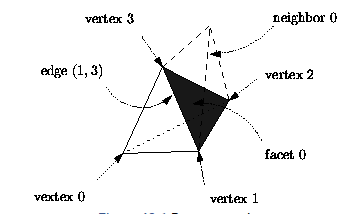
\includegraphics[width=0.5\textwidth]{figures/tetrahedron_cgal.png}
  \caption{Structure of a tetrahedron in CGAL}
  \label{fig::tetrahedron_cgal}
\end{figure}

A tetrahedron is represented through four entities :
\begin{itemize}
  \item Vertex: contains a point (3D coordinates)
  \item Edge: contains two vertices in specifi order and a cell
  \item Facet (face): stored thanks to a cell and the vertex facing it
  \item Cell: a tetrahedron giving access to four vertices and four adjacent celles
\end{itemize}

It is crucial to understand the structure provided by GAL because it will be
 necessary to access various parts of a tetrahedron. For example, when we work on
 edges to look for the interface, we need to know the vertices it contains.

\subsection{Displaying Method}

To display the proteins and the interface, we chose the \textit{.off } files
 which allow to store a list of points (colored or not) and to indicate the links between
  each of these points (to see figure \ref{fig::off_file}).

\begin{figure}[ht]
\centering
  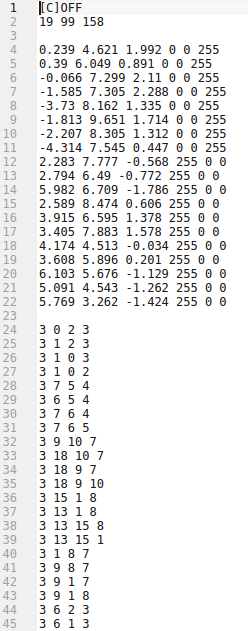
\includegraphics[width=0.3\textwidth]{figures/off_file.png}
  \caption{Example of a \textit{.off} file}
  \label{fig::off_file}
\end{figure}

The first line indicates the type of the file ( OFF) and the presence of coloring: [C]
The second line gives, in this order, the number of
 points, the number of cells and the number of edges, the
 latter not being necessary to reading the file. In our example, the lines 4 to 22
  list the coordinates of the points and the color associated with each.
  The color is stored in RGB (Red, Green, Blue) with integers between 0 and 255 or
   floats between 0.0 and 1.0.

Beyond the line 23, the cells are listed, with coming first an integer on every line giving
 the number of points of the cell. Since our example represents Delaunay triangulation,
 this number is worth 3 because every face of the triangulation corresponds
  to a triangle (it will not be valid any more for the surface faces which can contain
   any number of points). Following this integer come the indexes of the points forming
    the cell (or the face). This index corresponds to the rank of the point in the coordinates
     listed above.

     Finally, thanks to the CGAL library and this visualisation method, we were able
     to implement the theoretical method described previously.
